% Chapter for alternative methods to solving the problem.

\chapter{Methods}
\label{ch:methods}

In this Section, I discuss my solution to the problem stated in Chapter
\ref{ch:intro} and various alternatives I considered along the way. First I will
briefly introduce the schematic entry GUI. Next, I will discuss in detail how
we solved the protoboard layout problem and how we evaluated our solution.

\section{GUI}

We designed the schematic entry GUI to have a rich set of features so as to make
drawing schematics a very easy and intuitive task for students.
Figure \ref{fig:gui_example} gives a version of the schematic drawn in Figure
\ref{fig:schematic} as drawn of the schematic entry tool. Appendix \ref{app:gui}
discusses the features and capabilities of the schematic entry GUI in much
further detail.

\begin{figure}
\begin{center}
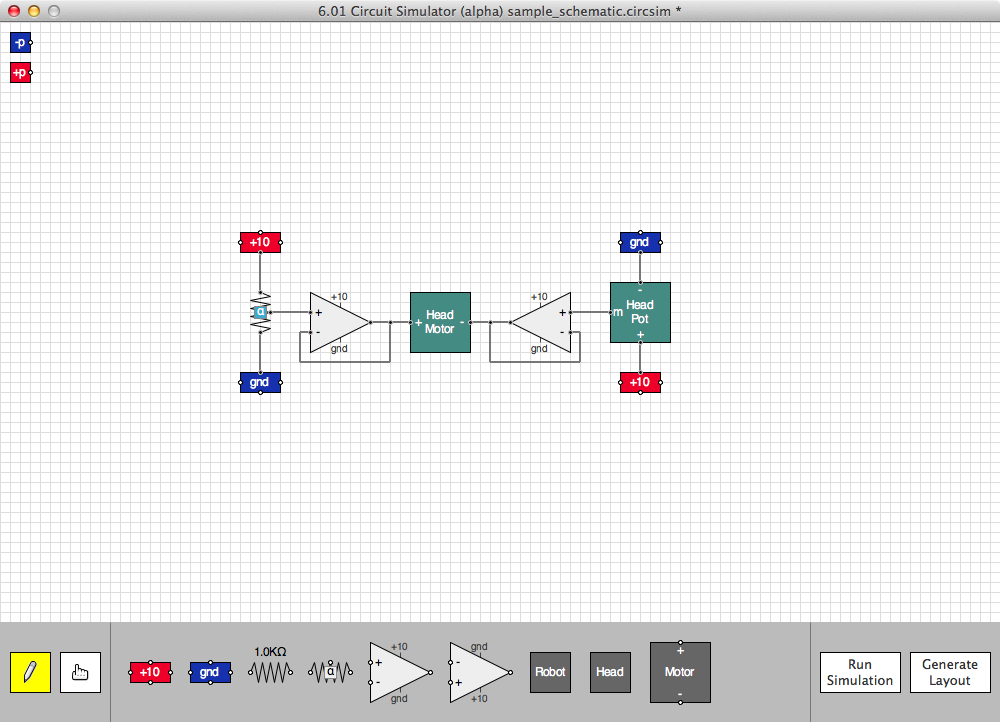
\includegraphics[width=\textwidth]{Images/gui_example.png}
\caption{TODO}
\label{fig:gui_example}
\end{center}
\end{figure}

\section{Solving the Layout Problem}

I solved this problem by formulating it as a search problem. By this I mean,
given a schematic of a circuit, I start from an empty protoboard, and I search
through the space of all possible protoboard layouts to find the protoboard
corresponding to the schematic at hand. The space of all possible protoboards is
very large \q, so I utilize various simplifications
and heuristics to facilitate the search.

I broke down the problem into two parts. The first task is finding a placement
of all the circuit pieces on the protoboard. The second task is wiring them up
appropriately.

\subsection{Part 1: Piece Placement}
\label{sec:placement}

Let us first consider how to place a set of circuit pieces on the protoboard for
a given circuit schematic. Any given circuit may contain resistors, Op Amps,
pots, motors, head connector parts, or robot connector parts. For each of these
components, we must put down a corresponding piece on the protoboard. As each
piece may be placed on the protoboard in one of many different ways, I first
decided on a fixed set of allowed placements for each of the pieces. Figure
\ref{fig:piece_placement} presents these acceptable placements.
Resistors are placed in the middle strip of the protoboard. Op Amp pieces are
also placed in the middle strip of the protoboard, but with two possible
orientations. Op Amp pieces are unique in that each Op Amp pieces contains two
Op Amps within it. Thus, we face the task of packaging the Op Amps in the
schematic in the ``best" possible way, i.e. so as to require as little work as
possible when wiring the pieces together. Section \ref{sec:justify_placement}
more precisely discusses the number of possibilities. Pots have two possible
vertical positions as well as two possible orientations.
The connector pieces have two possible vertical positions each.

\begin{figure}
\begin{center}
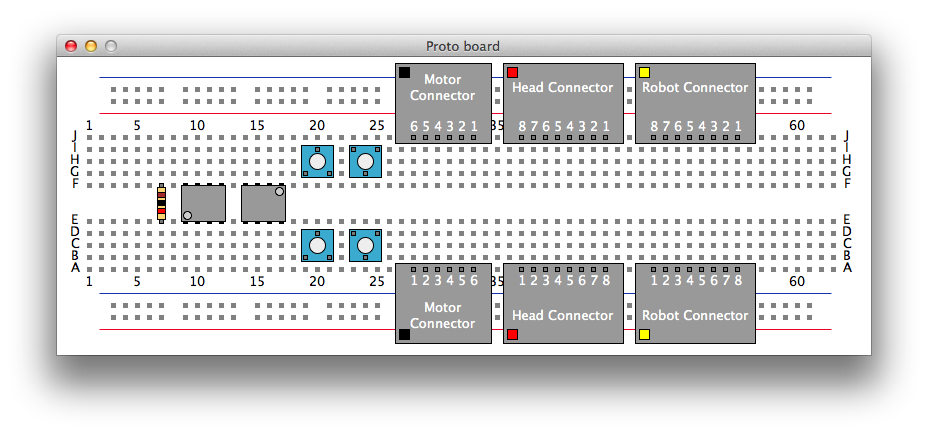
\includegraphics[width=\linewidth]{Images/piece_placement_options.png}
\caption{Various acceptable ways of putting each of the circuit pieces on the
protoboard.}
\label{fig:piece_placement}
\end{center}
\end{figure}

When choosing a placement of circuit pieces on the protoboard, we have at hand a
plethora of options. First we must choose among a possibly large number of ways
to package together the Op Amps in the circuit. For each possible packaging of
Op Amps, we must consider various ways of placing the pieces on the protoboard,
even with the restrictions put forth above.

\subsubsection{Simplifications}

I reduce this large number of options by only allowing placements in which no
two pieces share a column. This is not necessary in general, but the
number of pieces necessary for a typical 6.01 circuit would certainly fit in
this framework.

Next, I specify that there be exactly two columns on the protoboard separating
each consecutive pair of pieces, unless the pieces are both resistors, in which
case there must be exactly one column separating them. These numbers of columns
were chosen to leave enough space for wiring. Given a set of pieces to be put on
the protoboard, this specification reduces the
problem of choosing a placement for the pieces to finding an \emph{order} of the
pieces together with choosing their respective vertical locations and
orientations.

Given these simplifications, we have various options as to how to pick a
placement.

\subsubsection{Random Placement}

One simple alternative may be to choose a placement randomly. That is, we choose
an Op Amp packaging randomly; we choose an order of the pieces randomly; and we
choose the vertical locations and orientations of the pieces randomly as well.
The advantage of this
approach is that it gives us a placement very quickly without requiring much
computation. On the other hand, we may end up placing two pieces that need to be
connected to each other very far apart, and we will have a difficult time doing
the wiring. Hence, we ought to consider alternatives in which we take into
account the task of wiring. We should try to place the pieces so as to require
as little work during wiring as possible.

\subsubsection{Minimal Heuristic Cost}

The key idea is that if two pieces are meant to be connected together by wires,
then they ought to be placed close to each other on the protoboard. We can
capture this idea by assigning heuristic costs to the placements and choosing
a placement that produces the minimal heuristic cost. To this end, there are two
heuristic cost functions we considered.

\paragraph{Distance Based Cost}
Given a circuit
schematic and a corresponding placement of the circuit pieces on the protoboard,
what do we need to connect with wires? Well, every pair of components in the
schematic that are connected by a wire gives us a corresponding pair of
locations on the protoboard that ought to be connected by wires. However, we can
express this requirement a little bit more concisely. We ought to consider all
of the nodes in the schematic, and find the circuit components in the schematic
that are connected to the respective nodes. Now for each node in the circuit, we
get a set of locations on the protoboard that ought to be interconnected. The
first step in devising the distance based cost function is to have a way to
estimate the cost of connecting two locations on the protoboard. A simple such
cost function that comes to mind is the Manhattan distance between the two
locations. Recall that we want to produce aesthetically pleasing protoboard
layouts, and one of the requirements in achieving this goal is only using
horizontal and vertical wires (i.e. no diagonal wires) so the Manhattan distance
cost is appropriate. Given this heuristic cost for connecting two locations with
wires, we can define the heuristic cost for interconnecting the locations
associated with a particular node to be the weight of the minimum spanning tree
of the locations. Now we can define the cost of a placement to be the sum over
all nodes in the circuit of the cost for interconnecting the locations for each
node.

\paragraph{Blocking Based Cost}
The most scare resource on the protoboard are the rows. We are given $10$ rows
with which to work, and in producing a layout, we must fit all the wires within
these $10$ rows. This gives us an idea on how to define how hard a placement
will be to wire. Given a set of pieces, we can find a set of pairs of locations
on the board that need to be connected as we did above.
As noted in Section \ref{sec:what_is_protoboard} there are two groups of $5$
rows on a protoboard. Now for each group of rows and each column in the group of
rows, we can count how many pieces reside in that column, and how many wires may
pass through the column (in connecting a given pair of locations assuming an
empty protoboard). Our goal will be to minimize the number of columns that
would be used heavily. In our implementation, the final cost is computed as
the sum of the squares of the counts for each column.

Using one of the two cost functions discussed above, we can aim to find a
placement with the minimal cost. However, this involves trying all possible
orderings of the pieces with which we are working. For example, if we are trying
to order $10$ pieces, we would need to look at $10! = 3628800$ possible
orderings \q. Note that this is in addition to
searching over all possible ways
of packaging the Op Amps together. It is clear to see that the search for a
minimal cost placement quickly gets out of hand. So we aim to find a placement
that has a very small, though maybe not minimal, cost.

\subsubsection{Small Heuristic Cost}

Algorithm \ref{alg:small_cost_placement} presents a polynomial-time procedure
that orders a
given list of pieces in a way that results in a small cost. The algorithm places
one of the pieces at a time, starting from an empty placement. It relies
on two ideas. First, once a piece has been placed, all the pieces that are
connected to it will be placed soon after so that it is more likely that those
pieces are placed close to it. Second, we place the pieces with the most nodes
first since those are the ones that most likely have connections with many other
pieces.

\begin{algorithm}
\KwData{A list $P$ of circuit pieces.}
\KwResult{A list $R$ of circuit pieces representing a placement.}
\BlankLine
Sort $P$ in decreasing number of nodes on the respective pieces\\
$Q$ $\leftarrow$ empty Queue\\
$R$ $\leftarrow$ empty List\\
\While{$P$ is not empty}{
Pop the first piece in $P$ and push it onto $Q$\\
\While{$Q$ is not empty}{
$p$ $\leftarrow$ $Q$.pop()\\
Consider all vertical locations and orientations of $p$\\
Place $p$ at an index in $R$ that minimizes the cost of $P$\\
\ForEach{piece $q$ in $P$ connected to $p$}{
Pop $q$ out of $P$ and push it onto $Q$\\
}}}
\caption{Producing a circuit piece placement with small heuristic cost.}
\label{alg:small_cost_placement}
\end{algorithm}

Using one of the above methods, we can find a placement of circuit pieces on a
protoboard. Our next task is wiring them together to produce a circuit
equivalent to the circuit schematic of interest.

\subsection{Part 2: Wiring}

In the previous section we discussed what locations we need to wire together:
for every node in the circuit, we get a set of locations on the protoboard that
need to be interconnected. The question now is how to achieve this wiring. We
approach the problem as a search problem and use the $A*$ search algorithm to
solve it. In fact the wiring step uses an infrastructure for the $A*$ search
algorithm exactly as presented in the Search module of 6.01. Hence students in
the class may very much appreciate an application of something they learned
earlier in the course to produce a tool that they are using for something that
may seem completely unrelated.

\subsubsection{Using $A*$}

When using the $A*$ algorithm, we need to design four things:

\begin{enumerate}
\item The notion of a vertex\footnote{The preferred name is ``node" but I will
use vertex since we already use node to refer to nodes in circuits.} in the
search tree, the cost associated with a vertex, and how we obtain the neighbors
of a vertex,
\item The starting vertex,
\item How we identify whether a particular vertex in the search tree achieves
the goal of the search, and
\item A heuristic function that estimates the distance from a given vertex to a
goal vertex.
\end{enumerate}

\subsubsection{Vertices}

Each vertex will hold a representation of some protoboard. Each representation
will contain all of the pieces, and possibly a set of wires interconnecting the
pieces. The starting vertex will have all of the pieces but no wires.

We obtain the neighbors of a vertex by taking the current protoboard and
producing new ones in which we place exactly one wire at various locations. We
choose the starting point of a wire to be any one of the free locations on the
protoboard that is already connected to one of the pieces, and we extend the
wires in all possible vertical and horizontal directions up to some fixed wire
length. Note that we need
to take great care when placing wires in order not to short different nodes. We
discard any vertices that arise from placing a wire that shorts two different
nodes.

The way we define the cost of a vertex, i.e. the cost of getting from the
starting vertex to a vertex of interest, depends on what we consider to be an
aesthetically pleasing protoboard layout. In general, we want to penalize having
long wires, many wires, or crossing wires. In my implementation, while I have
a large penalty for two crossing wires of opposite orientations (i.e. vertical
and horizontal), I do not allow crossing wires that have the same orientation as
this configuration is particularly difficult to physically build and debug.
Finally, we want to favor making a desired interconnection between locations
on the protoboard. I chose my penalties experimentally
\q.

Each vertex will not only hold a protoboard, but it will also hold a set of
pairs of locations on the protoboard that need to be connected by wires. Each
pair $(loc_1, loc_2)$ of locations tells us that we need to have a set of wires
connecting some location connected to $loc_1$ to some location connected to
$loc_2$.

An important consideration we need to make is how we want to organize the
search. Recall that we have a set of nodes in the circuit of interest, and for
each node we have a set of locations that need to be interconnected. Given this
information, we may choose one of the following three strategies to carryout the
search:

\begin{enumerate}
\item All pairs: For each node, collect a set of pairs of locations on the
protoboard
corresponding to a minimum spanning tree of the locations for that node, so that
if all pairs of locations in this spanning tree are connected, then the
locations for the node will be interconnected. Collect all such pairs of
locations for all of the nodes in the circuit, and have the starting vertex hold
this set of pairs of locations.
\item Per-node: Treat each node separately. That is, iteratively interconnect the
locations for each of the nodes until there are no more nodes in the circuit.
\item Per-pair: Treat each pair of locations that needs to be connected
separately. That
is, iteratively connect pairs of locations that need to be connected until there
are no more pairs.
\end{enumerate}

The choice of one of these strategies has a significant effect on the outcome of
the search. We will discuss the difference in detail in Chapter
\ref{ch:results}.

\subsubsection{Goal test}

Given a vertex, we know that it is a goal vertex if all of the pairs of
locations it holds are already connected in the protoboard it holds.

\subsubsection{Search heuristic}

In $A*$ search, choosing the right heuristic can often make the search much more
efficient. In our problem, one option we have is not to use a heuristic, and
that alternative will be explored in Chapter \ref{ch:results}. However there is
a natural heuristic that suggests itself that we ought to consider. Given a
vertex, we can estimate its distance from a goal as follows. For each pair of
locations $(loc_1, loc_2)$ that need to be connected, we could consider its
distance from the
goal to be the smallest Manhattan distance between any location connected to
$loc_1$ and any other location connected to $loc_2$. To compute the heuristic
cost of a vertex, we simply add up this value for each of the pairs of locations
that need to be connected. Chapter \ref{ch:results} presents the performance of
this heuristic verses using no heuristic.

\subsection{Combining the methods}
\label{sec:combined_alg}

With the methods discussed so far, we aimed to completely solve the layout problem
with one placement method and one wiring method. However, as we will soon see,
such an algorithm is bound to fail on some set of schematics. When we ultimately
put the final algorithm in front of students, we would like to avoid failure.
The algorithm should always be able to generate layouts. Generating a layout
with a few diagonal or crossing wires is better than silently failing and leaving
the student empty handed. Here, we will discuss how we combine the methods
described so far into one layout algorithm. The motivation for this combination
will be discussed in Chapter \ref{ch:discussion} based on the data we obtain
for the alternatives described above. Algorithm \ref{alg:combined} presents the
combination algorithm.

\begin{algorithm}
\KwData{A circuit schematic $C$.}
\KwResult{A layout corresponding to $C$.}
\BlankLine
\ForEach{Placement cost metric $M$ in (DISTANCE, BLOCKING)}{
$P$ $\leftarrow$ Placement for $C$ by using cost metric $M$.\\
\ForEach{Order $O$ in (INCREASING, DECREASING)}{
$pairs$ $\leftarrow$ Pairs of location on $P$ to connect given schematic $C$ and connection order $O$.\\
\ForEach{$(loc_1, loc_2)$ in $pairs$}{
Attempt to connect $loc_1$ and $loc_2$ on $P$.\\
If successful, update $P$ accordingly and then post-process $P$.\\
If not, record that the pair $(loc_1, loc_2)$ was not successfully connected.\\
}
If all pairs are successfully connected, post-process and return $P$.\\
}}
Pick ``best" unfinished layout.\\
Connect remaining pairs with shortest possible wires (possibly diagonal).\\
Post-process and return resulting layout.\\
\caption{Layout algorithm obtained by combining multiple ideas.}
\label{alg:combined}
\end{algorithm}

There are a few key items in Algorithm \ref{alg:combined}. The algorithm works
by attempting to solve the problem in four different ways: two different ways of
doing placement together with two different orders of wiring pairs. Note,
therefore, that we have chosen per-pair wiring. If any one of the four trials
succeeds, the algorithm immediately returns the corresponding layout. If all
four trials fail, on the other hand, the algorithm picks the ``best" partial
solution and completes that solution by placing possibly diagonal wires, ``best"
being the partial solution that would require the least amount of additional
wiring. This last step makes it highly unlikely that the algorithm will ever fail.
The only way for the algorithm to fail is for there to be two nodes that need to be
connected where all of the protoboard locations for at least one of the nodes is
occupied, which is highly unlikely to happen. This high success rate comes at the
cost of placing wires that will almost surely cross other wires on the board.

The algorithm also has a post-processing step that attempts to to improve the
layout. The post-processing step makes three types of simple changes to the
layout. First, we throw away any wires that do not serve to connect two parts
of the circuit. That is, we throw away wires which have one end connected to
the circuit, and the other end connected to nothing at all. This could happen
in the search done by the wiring step, though very rarely. Second, we truncate
long vertical wires into an equivalent set of smaller wires. For example, a wire
going from one of the top rails to one of the bottom rails can be replaced by
three smaller wires making the same connection. This change frees up rows for
subsequent connections. Finally, if shifting a horizontal wire up or down
results in fewer wire crosses, we make that change.

The last important aspect of this final algorithm not explicitly stated in
Algorithm \ref{alg:combined} is that, as it is the algorithm that will be put
in front of students, it will be allowed to use wires of a select few lengths.
The kits that students work with certainly do not come with wires of all lengths,
so we force the wiring step to use wires of only those allowed lengths.

\subsection{Evaluation Method}

Here we present how we go about evaluating a particular solution to the problem.
How can we tell if a layout tool is good? In particular, how can we tell if a
layout tool is good enough for the purposes of 6.01 labs. To answer these
questions well, we need to test the layout tool on numerous schematics and
analyze its performance on laying out those schematics. As manually generating
numerous test schematics is tedious and very time-consuming, we devised a method
to randomly generate thousands of test schematics.

The random schematic generation goes as follows. We create $6$ basic sub-parts
of schematics. These $6$ bases are depicted in Figure
\ref{fig:random_gen_bases}. These bases cover all of the components that may be
necessary in a 6.01 circuit. Each sub-part also offers at least $3$ points of
connection with other subparts. The random generation algorithm takes all
possible combinations of
$6$ bases, allowing for repetition of bases with some restrictions.
The Head Connector and Robot Connector bases can appear at most once as there is
no need for more than one of each of these in 6.01 labs. The pot-follower base (
i.e. the base that contains one pot and a follower op amp) can appear at most
twice as we never need more than two pots in 6.01 circuits. The motor base can
also appear at most twice as we never need more than two motors per circuit in
6.01 labs. The other bases, T-resistor configuration and voltage divider, can be
repeated up to 6 times. For a given combination of bases, we generate up $n$
schematics, where $n$ depends on the number of bases in the configurations (
larger for configurations with more bases in them).
We generate the $n$ schematics by choosing a number of interconnections between
the bases from $0$ to $n-1$. For each number of interconnections, we generate
a schematic in which we put that many randomly chosen wires interconnecting
the bases in the combination. Figure \ref{fig:example_random_schematic} presents
a sample randomly generated schematic.

\begin{figure}
\begin{center}
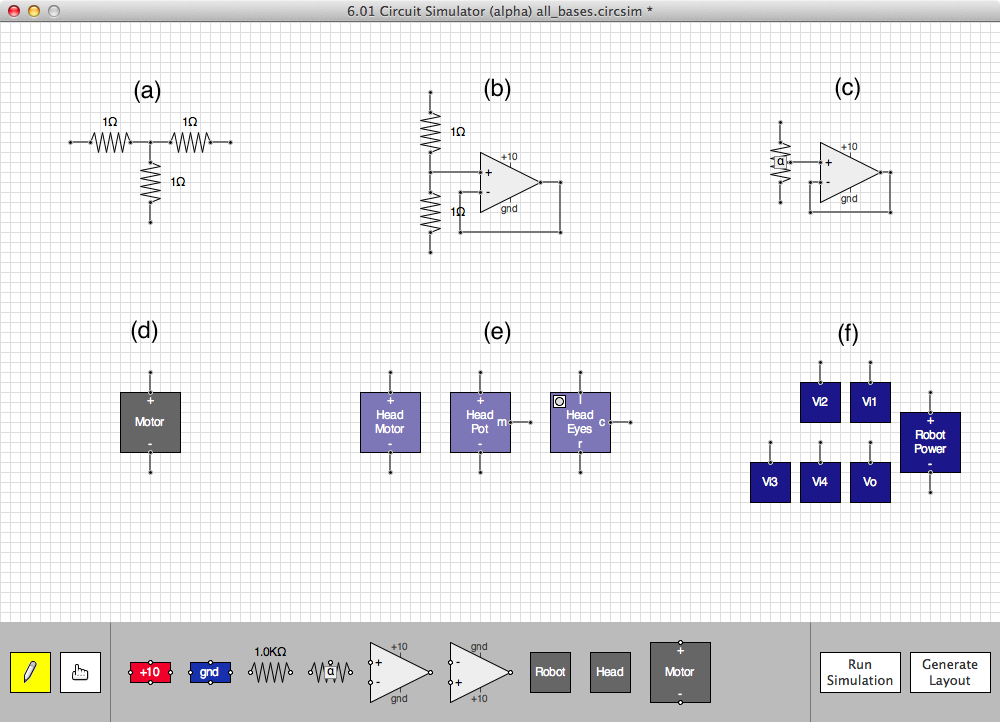
\includegraphics[width=\textwidth]{Images/auto_generation_bases.png}
\caption{Bases for random schematic generation.}
\label{fig:random_gen_bases}
\end{center}
\end{figure}

\begin{figure}
\begin{center}
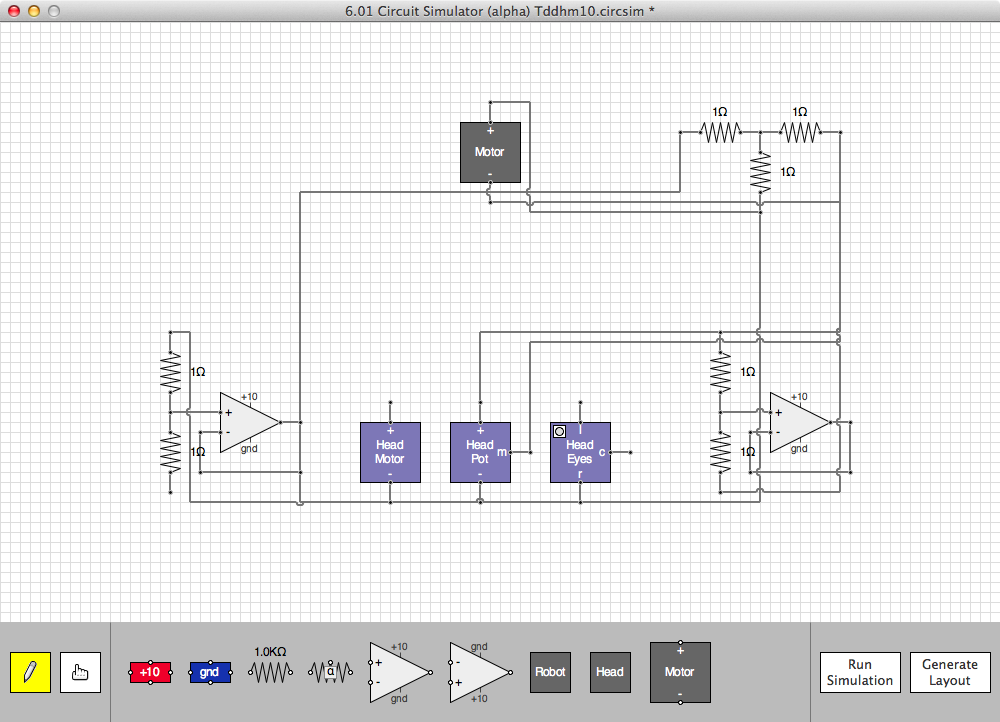
\includegraphics[width=\textwidth]{Images/auto_generation_example.png}
\caption{Sample randomly generated schematic.}
\label{fig:example_random_schematic}
\end{center}
\end{figure}

This scheme produces a total of $4425$ test schematics out of a possible total
of approximately $1.2e27$. When testing a particular algorithm on these test
schematics, we run the algorithm on each test schematic $10$ times. Chapter
\ref{ch:results} presents the data collected in this manner comparing the
various alternatives discussed in this Chapter.

An important question we must answer is how we quantify the goodness (or badness)
of a particular layout. Our approach takes a weighted sum of a particular set of
attributes of a given layout, where the weights are chosen comparatively. We set
the badness of a layout to be:
\begin{align*}
&1 \cdot NUMBER\_OF\_WIRES + \\
&10 \cdot TOTAL\_WIRE\_LENGTH + \\
&50 \cdot NUMBER\_OF\_WIRE\_CROSSES + \\
&100 \cdot NUMBER\_OF\_DIAGONAL\_WIRES + \\
&1000 \cdot NUMBER\_OF\_WIRE\_OCCLUSIONS + \\
&1000 \cdot NUMBER\_OF\_WIRE\text{-}PIECE\_CROSSINGS.
\end{align*}
We will use this metric to decide which of a given set of alternatives tends to
produce the better layouts.
